\chapter{系统设计}

\section{总体设计}
\label{sec:overalldesign}

本文主要参照Linux操作系统的内核框架,尝试实现一个带有文件操作功能和命令
行接口的简单操作系统。本系统主要包含以下四个模块:1)启动模块;2)进程
模块;3)数据存储模块;4)外围功能模块。

这四个模块分别有自己负责的范围。其中,启动模块负责从上电开机到操作系统
启动的过程;进程模块负责进程的产生、调度、和管理;数据存储模块实现硬盘、
内存等存储数据的功能,它是后续的文件系统、键盘输入等功能的基础;外围功
能模块建立在前三个模块的基础之上,主要是一些针对文件的操作,包括文件的
打开、关闭、读写、删除等等。这些功能的实现都离不开前三个模块,只有先完
成了前三个模块,才能实现这些基本的功能。

\section{模块设计}

\subsection{启动模块}

启动模块主要涉及BIOS、MBR、Loader、Kernel等部分。在操作系统启动过程中,
先由BIOS来找到MBR,
然后由MBR来引导并加载Loader,再由Loader来加载Kernel。如图
\ref{fig:boot}所示,启动模块的目的可以总结为一个,那就
是加载Kernel。它的详细过程在第\ref{cha:OSboot}章中将会介绍。

\begin{figure}[H]
  \centering
  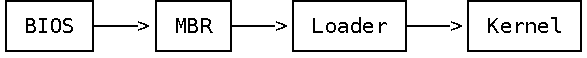
\includegraphics[width=.6\textwidth]{boot}
  \caption{与系统启动相关的各模块}
  \label{fig:boot}
\end{figure}

\subsection{进程模块}

进程模块主要包括特权级的转变、用户进程的创建、还有进程调度等方面。有了该模块操作系统才能使用户
程序在一个相对安全的环境中执行,并且能够实现多任务同时进行与切换。在本操作系统中,特权级转
变采用的是中断返回的方法:当中断发生时,在中断入口函数\texttt{intr\%1entry()}中通过\texttt{push}
操作来保存当前任务的上下文数据,因此,之后也需要有相应的\texttt{pop}操作来恢复数据,这属于
\texttt{intr\%1entry()}函数的逆过程,在使用\texttt{pop}操作恢复数据后,CPU就会认为用户进程从中断返回了。
在此操作之后,用户进程将在最低的特权级3下运行,操作系统处于最高特权级0,这样就达到了
该模块的目的。当用户进程处在特权级3之后,进程的创建就是通过一个\texttt{process\_execute()}函数来创建
的,创建成功后再由时钟中断用\texttt{schedule()}从就绪队列中进行调度。详细的步骤在第
\ref{sec:course}节中将会介绍。

\subsection{内存模块}

此模块就是为了进程而存在的,主要为新产生的进程分配对应的内存空间,在进程结束后再对内存进行
回收。内存的创建并不是提前准备好的,它是在需要的时候由程序动态创建的,例如进程需要内存的时
候,会调用相关的函数,然后动态分配并且维护内存块资源,再使用完内存后,还需要把内存回收回去,
而内存的使用情况一直是由位图\footnote{位图是操作系统中常用的一种数据结构,是一个二进制数
  组,其中的每个Bit表示相应的存储快的状态,通常用0表示未使用,1表示已使用。}来进行管理的,
所以无论内存的分配或者释放,本质上其实就是在设置相关位图的相应位,也就是在读写位图。

\subsection{外围功能模块}

在有了启动、进程、内存模块之后,就可以实现一个简单的文件系统,一个简单的shell,shell的一些
简单功能,本文中主要实现的功能有:文件的创建、文件的删除、文件的打开、文件的关闭、文件的写
入、文件的读取、文件的删除这些文件操作。

而在shell中实现了\Ctrl{L}和\Ctrl{U}快捷键,分别是清屏和清除输入,还有一些简单的\texttt{ls}、\texttt{cd}、
\texttt{mkdir}、\texttt{rmdir}操作。 

%%% Local Variables:
%%% mode: latex
%%% TeX-master: "../thesis"
%%% End:
